\chapter{Perspective}
%Brugbarheden af WOMBAT n�r man arbejder med b�rn med ASD
%Betydning af WOMBAT i forhold til b�rn med ASD


%\subsection{Making a Handset Version}
%It is, at the moment, not possible to install and run the WOMBAT application on an Android handset, but there are several reasons for considering making a handset version of the application aswell.
%
%\subsection{Better Graphics}
%
%
%\subsection{New Design Features}

\section{Future Work}
In this section we will list some ideas for further development on the WOMBAT application.

%-------------------------------Test changes----------------------------------------
\subsection{Ideas based on the usability and acceptance test}
In this subsection we will briefly describe changes we would like to implement based on the usability test and the acceptance test.

\subsubsection{Color picking}
WOMBAT is currently using a color palette that the guardians uses to pick colors, we would like to change this into a list of predefined colors and an advanced button where they are able to define new colors with a color palette. This change would ease the color picking.

\subsubsection{Gradient button}
The gradient button can be difficult to spot, it is therefore necessary to improve the layout. It might help if the button layout looks the same as all the other buttons in WOMBAT.

\subsubsection{Improve customize fragment buttons}
The buttons in WOMBAT need to be redesigned to appear more like buttons. The attachment buttons visual effect after attaching an attachment needs to be improved such that it is more clear for the user, when an attachment has been attached.

\subsubsection{Delete}
It is not intuitive how to delete a configuration. It might help to remove the long-click and make a delete button on each configuration. Figure: \ref{fig:futureworkDelete} illustrates how such a button might look like.


\begin{figure}[H]
	\centering
		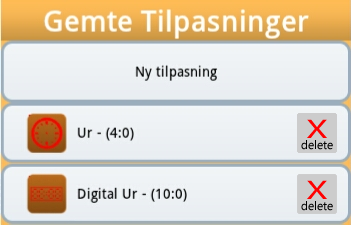
\includegraphics[scale=0.6]{Images/Discussion/delete.png}
	\caption{Illustration of possible delete button}
	\label{fig:futureworkDelete}
\end{figure}


\subsubsection{Last used and Predefined layout changes}
The usability test showed that the last used and predefined category were hard to find, these two categories need a design change to have a different layout than the children in the list. This could be achieved by changing the background color of these two categories.

\subsubsection{Done screen lock}
The acceptance test showed that it is necessary to improve the lock on the done screen picture. The done screen unlocks by a single touch on the screen, which is issue, would be changed to e.g. a long-click instead.

%-------------------------------Ideas----------------------------------------
\subsection{Ideas}
In this subsection we will briefly describe ideas which can be used for future development of WOMBAT.

\subsubsection{Handset Version}
It is, at the moment, not possible to install and run the WOMBAT application on an Android handset, but it might be more convenient to bring a handset than a tablet, when the guardians and children is on a trip.

\subsubsection{Improved Graphics}
WOMBAT is currently using canvas for drawing all the timers, which is simple 2D graphic. It is possible to improve the graphic by using OpenGL instead. OpenGL is used for drawing detailed 3D objects. The benefit of improving the graphic in WOMBAT is to make the timers more realistic and look like the timers which the children already uses. There have been conducted a comparison between canvas and OpenGL which can been read about in subsection: \ref{subsection:compare}.

\subsubsection{Overlay timers}
This idea is based on the second part of our original idea, that can be found in \autoref{sec:vision}.
When you exit the timer screen with a timer in progress, the timer will be destroyed. 
Instead of destroying the timer, it should enable an overlay timer which should continue from where the timer left off. 
The overlay timer should always appear on top of all the other application. 
This would make it possible for the guardian to conduct multiple tasks without stopping a timer. 
When the guardian enters WOMBAT again, it should remove the overlay and continue the timer normally.

\subsubsection{Code Architecture}
The draw feature which is a part of the \texttt{DrawLib}, were original designed to be a part of the \texttt{TimerLib}, the decision of this can be read in \autoref{sec:Architecture}. 
The ideal architecture would be to import the draw methods into each timer class, that way you could call the method on a certain timer object and return a \texttt{View}. 
By doing so, you would not have to check on which object you are handling, see \autoref{code:drawlibnow} and \autoref{code:drawlibfuture}.


\begin{figure}[H]
\begin{lstlisting}
...
			switch(sub.getAttachment().getForm()){
			case Timer:
				...
				break;
			case SingleImg:
				...
				break;
			case SplitImg:
				frameWidth = frameWidth/2;
				v = genDrawView(sub, frameWidth);
				frame.addView(v, frameWidth, frameHeight);
				frameWidth = frameWidth/2;
				frameWidth = frameWidth - 15;
				i = new ImageView(this);
				i.setImageResource(sub.getAttachment().getLeftImg().getPath());
				i.setBackgroundDrawable(gd);
				frame.addView(i, frameWidth, frameHeight);
				i2 = new ImageView(this);
				i2.setImageResource(sub.getAttachment().getRightImg().getPath());
				i2.setBackgroundDrawable(gd);
				frame.addView(i2, frameWidth, frameHeight);
				i3 = new ImageView(this);
				i3.setBackgroundDrawable(gd);
				frame.addView(i3, 30, frameHeight);
				break;
			}
			setContentView(frame);	
			...
\end{lstlisting}
\caption{Code snippet of how \texttt{DrawLib} checks for object form to generate the corresponding \texttt{View}.}%
\label{code:drawlibnow}%
\end{figure}

\begin{figure}[H]
\begin{lstlisting}
LinearLayout frame = new LinearLayout(this);
Guardian guard = Guardian.getInstance();
frame.addView(guard.getSubProfile().draw());
setContentView(frame);	
\end{lstlisting}
\caption{Example of how WOMBAT would generate timer \texttt{View}, if \texttt{DrawLib} was apart of \texttt{TimerLib}.}%
\label{code:drawlibfuture}%
\end{figure}

%\subsubsection{Child customize fragment}
%N�r man starter WOMBAT skal h�jre fragment vise noget brugbart information.
%N�r man klikker p� et barn skal det h�jre fragment �ndres til instillinger for det barn.
%N�r man s� klikker p� en subprofile skal det skifte til instillinger for den valgte subprofile.

\subsubsection{Last used}
WOMBAT do not save the configurations in the last used list, this is because it is not implemented to work together with \texttt{OasisLocalDatabase}. When the WOMBAT activity is destroyed or the memory of the device is cleared, the last used list will be empty. In the future this function should be reimplemented to work together with the \texttt{OasisLocalDatabase}.

\subsubsection{Delete and save}
There is a bug which occurs when you create three or more new timers on the same profile. When you try to delete these timers it will delete them randomly and might even force WOMBAT to crash due to it is trying to delete a non existing setting in the \texttt{OasisLocalDatabase}. This is a bug in the application that needs to be future developed on.
